\chapter{Potentiel chimique et mélanges}\label{ch:b2:chemical-potential}

En hiver, une saleuse répand du sel sur une route verglacée et la glace fond à
\qty{-10}{\celsius}~; le liquide de refroidissement d'un moteur de voiture, de l'eau additionnée d'un tiers
d'éthane-1,2-diol, ne gèle pas par les nuits de gel et ne bout pas sous un capot
brûlant. Une substance dissoute abaisse la température de congélation de son solvant et
élève sa température d'ébullition, et, pour des solutions diluées, d'une quantité qui
dépend du nombre de particules dissoutes et non de leur nature. L'outil qui
l'explique est le \omterm{def:b2:chemical-potential:chemical-potential}{potentiel chimique}, dérivée partielle de
l'\omterm{def:b2:reaction-free-energy:gibbs-energy}{enthalpie libre} par rapport à la quantité d'un constituant. Il indique
«~où chaque espèce veut aller~», entre phases et par réactions,
et il transforme les activités, que le volume de première année utilisait comme des recettes, en
grandeurs démontrées.

\begin{recall}
\Cref{ch:b2:reaction-free-energy}~: l'\omterm{def:b2:reaction-free-energy:gibbs-energy}{enthalpie libre} $G = H - TS$, $\dd G =
V\dd p - S\dd T + \Delta_r G\,\dd\xi$, le critère d'évolution $\Delta_r G\,
\dd\xi \leq 0$. Le volume de première année a écrit l'activité d'un gaz sous la forme
$p_i/p^\circ$, celle d'un soluté $c_i/c^\circ$, et 1 pour un solide pur ou un
solvant, en notant que, dans les solutions ioniques concentrées, les activités s'écartent
des concentrations, «~correction traitée dans le volume de deuxième année~». En
physique~: la loi des gaz parfaits, et $(\partial G/\partial p)_T = V$ pour un corps
pur.
\end{recall}

\begin{omfigure}

\includegraphics[width=0.58\linewidth]{images/book3/ai/b2-03-salt-spreader.jpg}

{\small Une saleuse répand du sel sur une route enneigée. Le sel se dissout
dans la mince pellicule d'eau qui recouvre la glace, et la solution gèle à une
température plus basse que l'eau pure~: la glace fond.}
\end{omfigure}

\section{Grandeurs molaires partielles}

Mélangeons \qty{50}{mL} d'eau et \qty{50}{mL} d'éthanol~: le volume du
mélange est inférieur à \qty{100}{mL}. Dans un mélange, une grandeur extensive n'est
pas la somme des contributions des corps purs~; chaque constituant
contribue selon son environnement.

\begin{definition}[Grandeur molaire partielle]\label{def:b2:chemical-potential:partial-molar}
Soit $X(T, p, n_1, \dots, n_k)$ une fonction d'état extensive d'une phase
contenant les quantités $n_1, \dots, n_k$. La \emph{grandeur molaire
partielle}\index{grandeur molaire partielle} du constituant $i$ est
\[
  \bar X_i = \left(\frac{\partial X}{\partial n_i}\right)_{T, p, n_{j \ne i}} ,
\]
c'est-à-dire la variation de $X$ par mole de $i$ ajoutée à une grande quantité du mélange,
à $T$, $p$ et autres quantités fixées. Pour $X = V$, c'est le \emph{volume molaire
partiel}\index{volume molaire partiel} $\bar V_i$.
\end{definition}

\begin{theorem}[Identité d'Euler]\label{thm:b2:chemical-potential:euler}
À $T$ et $p$ fixées, $X = \sum_i n_i\bar X_i$.
\end{theorem}

\begin{proof}
$X$ est extensive~: multiplier toutes les quantités de matière par $\lambda$ multiplie
$X$ par $\lambda$, ce qui s'écrit $X(T, p, \lambda n_1, \dots, \lambda n_k) = \lambda X(T, p, n_1,
\dots, n_k)$. Dériver par rapport à $\lambda$ en $\lambda = 1$, par
dérivation composée~: $\sum_i n_i\,\partial X/\partial n_i = X$.
\end{proof}

\begin{proposition}[Relation de Gibbs--Duhem]\label{prop:b2:chemical-potential:gibbs-duhem}
À $T$ et $p$ fixées, $\sum_i n_i\,\dd\bar X_i = 0$~; dans un mélange binaire,
$x_1\dd\bar X_1 + x_2\dd\bar X_2 = 0$. Les \omterm{def:b2:chemical-potential:partial-molar}{grandeurs molaires partielles} des
constituants ne peuvent pas varier indépendamment.
\end{proposition}

\begin{proof}
À $T$, $p$ fixées, $\dd X = \sum_i\bar X_i\dd n_i$ par définition~; l'identité
d'Euler, différentiée, donne $\dd X = \sum_i\bar X_i\dd n_i + \sum_i
n_i\dd\bar X_i$. Il reste à soustraire.
\end{proof}

\begin{omfigure}
\begin{tikzpicture}
\begin{axis}[
  width=0.62\linewidth, height=5.4cm, xmin=0, xmax=1, ymin=8, ymax=62,
  axis x line=bottom, axis y line=left, xlabel={fraction molaire $x_2$},
  ylabel={volume molaire $V_m$ (modèle)}, xtick={0,0.2,0.4,0.6,0.8,1}, ytick=\empty,
  tick label style={font=\small}, label style={font=\small}, ylabel shift=10pt, clip=false]
\addplot[omDef, very thick, domain=0:1, samples=60] {18*(1-x) + 58*x - 25*x*(1-x)};
\addplot[black!40, dashed, domain=0:1] {18*(1-x) + 58*x};
\addplot[omThm, thick, domain=0:1] {14 + 35*x};
\fill[omThm] (axis cs:0.4,28) circle (1.6pt);
\node[omThm, anchor=east, font=\small] at (axis cs:-0.01,14) {$\bar V_1$};
\node[omThm, anchor=west, font=\small] at (axis cs:1,49) {$\bar V_2$};
\node[font=\scriptsize, anchor=south east, black!60] at (axis cs:0.62,44) {somme des volumes purs};
\node[font=\small, anchor=north west] at (axis cs:0.41,27) {$x_2 = 0.4$};
\end{axis}
\end{tikzpicture}

{\small La construction de la tangente. Le volume molaire d'un mélange binaire modèle
(en bleu) se situe au-dessous de la droite qui joint les volumes purs~: le mélange
se contracte. La tangente en une composition coupe les deux bords aux \omterm{def:b2:chemical-potential:partial-molar}{volumes molaires
partiels} $\bar V_1$ et $\bar V_2$ de cette composition.}
\end{omfigure}

\begin{method}[Grandeurs molaires partielles à partir d'une courbe]\label{met:b2:chemical-potential:tangent}
Tracer la grandeur molaire $X_m = X/(n_1 + n_2)$ en fonction de $x_2$. À la
composition étudiée, tracer la tangente~: elle coupe l'axe $x_2 = 0$ en
$\bar X_1$ et l'axe $x_2 = 1$ en $\bar X_2$. (Démonstration~: $X_m = x_1\bar X_1 +
x_2\bar X_2$ et, d'après Gibbs--Duhem, $\dd X_m/\dd x_2 = \bar X_2 - \bar X_1$.)
\end{method}

\section{Le potentiel chimique}

\begin{definition}[Potentiel chimique]\label{def:b2:chemical-potential:chemical-potential}
Le \emph{potentiel chimique}\index{potentiel chimique} du constituant $i$ dans
une phase est son \omterm{def:b2:reaction-free-energy:gibbs-energy}{enthalpie libre} molaire partielle,
\[
  \mu_i = \left(\frac{\partial G}{\partial n_i}\right)_{T, p, n_{j\ne i}} ,
\]
en \unit{J/mol}. Sa valeur lorsque $i$ est dans son état standard est son
\emph{potentiel chimique standard}\index{potentiel chimique standard}
$\mu_i^\circ(T)$, égal à l'\omterm{def:b2:reaction-free-energy:gibbs-energy}{enthalpie libre} molaire standard de $i$.
\end{definition}

Pour une phase dont les quantités peuvent changer (par réaction, ou par échange avec
une autre phase),
\[
  \dd G = V\dd p - S\dd T + \sum_i\mu_i\,\dd n_i ,\qquad G = \sum_i n_i\mu_i ,
\]
la seconde relation découlant de l'identité d'Euler. Avec une seule réaction, $\dd n_i =
\nu_i\dd\xi$, et par comparaison avec la \cref{prop:b2:reaction-free-energy:dG}~:
\[
  \Delta_r G = \sum_i\nu_i\mu_i .
\]
L'\omterm{def:b2:reaction-free-energy:reaction-gibbs}{enthalpie libre de réaction} est le bilan des \omterm{def:b2:chemical-potential:chemical-potential}{potentiels chimiques} des
produits et des réactifs.

\begin{theorem}[Équilibre entre phases]\label{thm:b2:chemical-potential:phase-equilibrium}
Un constituant présent dans deux phases $\alpha$ et $\beta$ d'un système fermé à
$T$ et $p$ uniformes est en équilibre entre elles si et seulement si
$\mu_i^\alpha = \mu_i^\beta$. Sinon, il passe spontanément de la
phase où son \omterm{def:b2:chemical-potential:chemical-potential}{potentiel chimique} est le plus élevé à celle où il est le plus bas.
\end{theorem}

\begin{proof}
Le transfert $i^\alpha \to i^\beta$ est une «~réaction~» avec $\nu^\alpha = -1$,
$\nu^\beta = +1$, donc $\Delta_r G = \mu_i^\beta - \mu_i^\alpha$. D'après le
critère d'évolution, il progresse ($\dd\xi > 0$) seulement si $\mu_i^\beta <
\mu_i^\alpha$, régresse si $\mu_i^\beta > \mu_i^\alpha$, et est à
l'équilibre s'ils sont égaux.
\end{proof}

Le \omterm{def:b2:chemical-potential:chemical-potential}{potentiel chimique} joue pour la matière le rôle que la température joue
pour la chaleur~: la chaleur va du chaud vers le froid, une espèce du haut vers le bas de l'échelle des $\mu$.

\section{Systèmes idéaux et activités}

\begin{proposition}[Potentiel chimique d'un gaz parfait]\label{prop:b2:chemical-potential:mu-gas}
Dans un mélange de gaz parfaits, un gaz de pression partielle $p_i$ a pour \omterm{def:b2:chemical-potential:chemical-potential}{potentiel chimique}
\[
  \mu_i = \mu_i^\circ(T) + RT\ln\frac{p_i}{p^\circ} .
\]
\end{proposition}

\begin{proof}
Pour une mole de gaz parfait pur, $(\partial\mu/\partial p)_T = V_m =
RT/p$~; l'intégration de $p^\circ$ à $p$ donne $\mu = \mu^\circ + RT\ln(p/p^\circ)$.
Dans un mélange de gaz parfaits, chaque gaz se comporte comme s'il était seul dans le volume, à
sa pression partielle~: il suffit de remplacer $p$ par $p_i$.
\end{proof}

\begin{definition}[Mélange idéal, solution diluée idéale]\label{def:b2:chemical-potential:ideal-mixture}
Un mélange liquide (ou solide) est un \emph{mélange idéal}\index{melange ideal@mélange idéal}
si, pour tout constituant et toute composition,
$\mu_i = \mu_i^*(T, p) + RT\ln x_i$, où $\mu_i^*$ est le \omterm{def:b2:chemical-potential:chemical-potential}{potentiel chimique}
du liquide pur $i$. Une solution est une \emph{solution diluée
idéale}\index{solution diluee ideale@solution diluée idéale} si le solvant obéit à cette loi et si chaque
soluté obéit à $\mu_j = \mu_j^\circ(T) + RT\ln(c_j/c^\circ)$, avec un état
standard qui est une solution hypothétique à $c^\circ = \qty{1}{mol/L}$ se comportant
comme si elle était infiniment diluée.
\end{definition}

Des molécules de taille et de forme voisines, dont les interactions ne dépendent pas
du partenaire (benzène et toluène, deux formes isotopiques d'une molécule), forment
des mélanges presque idéaux~; les solutions diluées se comportent idéalement parce que chaque particule
de soluté n'est entourée que de solvant.

\begin{theorem}[Loi de Raoult]\label{thm:b2:chemical-potential:raoult}
Au-dessus d'un mélange liquide idéal, la vapeur étant un gaz parfait, la pression
partielle de chaque constituant est proportionnelle à sa fraction molaire dans le
liquide~: $p_i = x_i\,p_i^*$, où $p_i^*$ est la pression de vapeur du liquide
pur à la même température (\emph{loi de Raoult}\index{loi de Raoult}).
\end{theorem}

\begin{proof}
À l'équilibre, $\mu_i(\text{liquide}) = \mu_i(\text{vapeur})$~: $\mu_i^* +
RT\ln x_i = \mu_i^\circ + RT\ln(p_i/p^\circ)$. Pour le liquide pur ($x_i = 1$,
$p_i = p_i^*$)~: $\mu_i^* = \mu_i^\circ + RT\ln(p_i^*/p^\circ)$. Par soustraction,
$RT\ln x_i = RT\ln(p_i/p_i^*)$. (On néglige la faible dépendance de $\mu_i^*$ en
la pression.)
\end{proof}

\begin{proposition}[Loi de Henry]\label{prop:b2:chemical-potential:henry}
Pour un soluté $j$ dilué en équilibre avec sa vapeur, $p_j = k_{H,j}\,x_j$
(ou $c_j = H_j\,p_j$)~: la pression partielle d'un soluté dilué est
proportionnelle à sa quantité dans la solution (\emph{loi de
Henry}\index{loi de Henry}). La \emph{constante de Henry}\index{constante de Henry}
$k_{H,j}$ dépend du soluté, du solvant et de la température~; ce n'est pas
la pression de vapeur du soluté pur.
\end{proposition}

\begin{proof}
Égaler $\mu_j^\circ(\text{solution}) + RT\ln(c_j/c^\circ)$ et
$\mu_j^\circ(\text{gaz}) + RT\ln(p_j/p^\circ)$~: $c_j/p_j$ est une fonction de $T$
seule. La constante contient les interactions de $j$ avec le solvant, non
avec lui-même.
\end{proof}

\begin{omfigure}
\begin{tikzpicture}
\begin{axis}[name=a,
  width=0.48\linewidth, height=5.6cm, xmin=0, xmax=1, ymin=0, ymax=1.5,
  axis x line=bottom, axis y line=left, xlabel={$x_1$}, ylabel={$p/p_1^*$},
  xtick={0,0.5,1}, ytick={0,0.5,1,1.5},
  tick label style={font=\small}, label style={font=\small}, title={\small idéal}]
\addplot[omDef, thick] table[x=x1, y=p1] {figdata/out/bachelor-2-raoult-henry-ideal.dat};
\addplot[omThm, thick] table[x=x1, y=p2] {figdata/out/bachelor-2-raoult-henry-ideal.dat};
\addplot[black, very thick] table[x=x1, y=p] {figdata/out/bachelor-2-raoult-henry-ideal.dat};
\node[omDef, font=\scriptsize, anchor=west] at (axis cs:0.55,0.42) {$p_1$};
\node[omThm, font=\scriptsize, anchor=west] at (axis cs:0.1,0.42) {$p_2$};
\node[font=\scriptsize, anchor=south] at (axis cs:0.5,0.8) {$p$};
\end{axis}
\begin{axis}[at={(a.east)}, anchor=west, xshift=1.2cm,
  width=0.48\linewidth, height=5.6cm, xmin=0, xmax=1, ymin=0, ymax=1.5,
  axis x line=bottom, axis y line=left, xlabel={$x_1$},
  xtick={0,0.5,1}, ytick={0,0.5,1,1.5},
  tick label style={font=\small}, label style={font=\small}, title={\small écart positif}]
\addplot[omDef, thick] table[x=x1, y=p1] {figdata/out/bachelor-2-raoult-henry-margules.dat};
\addplot[omThm, thick] table[x=x1, y=p2] {figdata/out/bachelor-2-raoult-henry-margules.dat};
\addplot[black, very thick] table[x=x1, y=p] {figdata/out/bachelor-2-raoult-henry-margules.dat};
\addplot[omDef, densely dashed, domain=0.6:1] {x};
\addplot[omDef, dotted, thick, domain=0:0.42] {3.004166*x};
\node[omDef, font=\scriptsize, anchor=west] at (axis cs:0.62,0.5) {Raoult};
\node[omDef, font=\scriptsize, anchor=east] at (axis cs:0.27,1.18) {Henry};
\node[omDef, font=\scriptsize, anchor=north west] at (axis cs:0.8,0.78) {$p_1$};
\node[omThm, font=\scriptsize, anchor=north] at (axis cs:0.55,0.24) {$p_2$};
\node[font=\scriptsize, anchor=south] at (axis cs:0.5,1.23) {$p$};
\end{axis}
\end{tikzpicture}

{\small Pressions de vapeur au-dessus d'un liquide binaire à température fixée, en unités
de $p_1^*$ (mélange modèle). À gauche, un \omterm{def:b2:chemical-potential:ideal-mixture}{mélange idéal}~: des droites (Raoult).
À droite, un mélange dont les molécules différentes s'attirent moins que les molécules
identiques~: les pressions sont au-dessus des droites idéales. Près de $x_1 = 1$, le constituant 1
suit la droite de Raoult (en tirets)~; près de $x_1 = 0$, il suit une droite de Henry
(en pointillés) de pente différente.}
% (computed in figdata/bachelor-2/raoult-henry.py; Margules parameter 1.1, model)
\end{omfigure}

\begin{example}[Le dioxyde de carbone d'un soda]\label{ex:b2:chemical-potential:soda}
À \qty{25}{\celsius}, la \omterm{prop:b2:chemical-potential:henry}{constante de Henry} du dioxyde de carbone dans l'eau vaut $H =
\qty{3.4e-4}{mol/(m^3.Pa)}$, soit \qty{0.034}{mol/(L.bar)}. Une bouteille
fermée sous \qty{4}{bar} de \ce{CO2} contient $0.034 \times 4 =
\qty{0.14}{mol/L}$ de gaz dissous, environ \qty{6}{g/L}. Une fois ouverte, le gaz
au-dessus d'elle est l'air, où $p_{\ce{CO2}} \approx \qty{4e-4}{bar}$~: la boisson est
dix mille fois sursaturée et pétille jusqu'à devenir plate.
% ledger: henry:CO2, air:CO2
\end{example}

\begin{proposition}[Activités et potentiels chimiques]\label{prop:b2:chemical-potential:activity}
Dans tous les cas rencontrés jusqu'ici, $\mu_i = \mu_i^\circ(T) + RT\ln a_i$, où $a_i$
est l'activité du volume de première année~: $p_i/p^\circ$ pour un gaz parfait,
$c_i/c^\circ$ pour un soluté dans une \omterm{def:b2:chemical-potential:ideal-mixture}{solution diluée idéale}, $x_i$ (proche de 1)
pour le solvant, et 1 pour un solide ou un liquide pur seul dans sa phase.
\end{proposition}

\begin{proof}
Pour le gaz et le soluté dilué, c'est le contenu de la
\cref{prop:b2:chemical-potential:mu-gas} et de la définition de la \omterm{def:b2:chemical-potential:ideal-mixture}{solution diluée
idéale}. Pour un constituant d'un \omterm{def:b2:chemical-potential:ideal-mixture}{mélange idéal}, on prend pour état standard
le liquide pur~: $a_i = x_i$, proche de 1 pour un solvant. Un solide ou un liquide
pur est son propre état standard (sa faible dépendance en la pression étant
négligée)~: $\mu = \mu^\circ$, $a = 1$.
\end{proof}

\begin{proposition}[Enthalpie libre de réaction et quotient]\label{prop:b2:chemical-potential:delta-g-q}
Pour une réaction $0 = \sum_i\nu_i\mathrm A_i$,
\[
  \Delta_r G = \Delta_r G^\circ(T) + RT\ln Q, \qquad Q = \prod_i a_i^{\nu_i} .
\]
\end{proposition}

\begin{proof}
$\Delta_r G = \sum_i\nu_i\mu_i = \sum_i\nu_i\mu_i^\circ + RT\sum_i\nu_i\ln a_i =
\Delta_r G^\circ + RT\ln\prod_i a_i^{\nu_i}$.
\end{proof}

C'est le pont entre l'\omterm{def:b2:reaction-free-energy:gibbs-energy}{enthalpie libre} du \cref{ch:b2:reaction-free-energy}
et le quotient de réaction du volume de première année. Le chapitre suivant le franchit.

\begin{method}[Choisir l'état de référence d'une activité]\label{met:b2:chemical-potential:activity-reference}
\begin{enumerate}
  \item Gaz~: le gaz parfait pur sous $p^\circ$~; $a = p_i/p^\circ$.
  \item Solvant, ou constituant d'un mélange de quantités comparables~: le
        liquide pur~; $a = \gamma_i x_i$ (référence de Raoult, $\gamma_i \to 1$
        quand $x_i \to 1$).
  \item Soluté~: la solution idéale à $c^\circ$~; $a = \gamma_j c_j/c^\circ$
        (référence de Henry, $\gamma_j \to 1$ à dilution infinie).
  \item Solide pur, liquide pur seul dans sa phase~: $a = 1$.
\end{enumerate}
\end{method}

\begin{history}[François-Marie Raoult]
\begin{minipage}[t]{0.2\linewidth}\vspace{0pt}
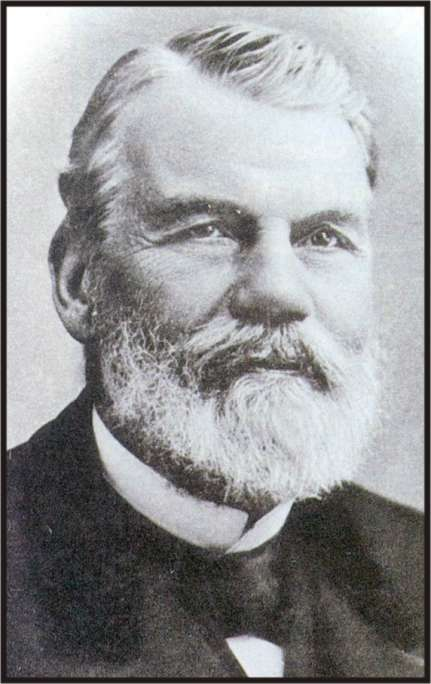
\includegraphics[width=\linewidth]{images/book3/raoult.jpg}
\end{minipage}\hfill
\begin{minipage}[t]{0.76\linewidth}\vspace{0pt}
François-Marie Raoult (1830--1901), professeur de chimie à Grenoble,
mesura dans les années 1880 les températures de congélation puis les pressions de vapeur
de centaines de solutions, et constata que, pour des solutions diluées, l'abaissement
dépend du nombre de molécules dissoutes et non de leur nature. Ses
mesures devinrent un moyen de «~peser~» les molécules, et appuyèrent la jeune
théorie des ions en solution. (Photographie~: domaine public, Wikimedia Commons.)
\end{minipage}
\end{history}

\section{Mélanges réels}

\begin{definition}[Coefficient d'activité]\label{def:b2:chemical-potential:activity-coefficient}
Dans un mélange réel, le \omterm{def:b2:chemical-potential:chemical-potential}{potentiel chimique} s'écrit $\mu_i = \mu_i^\circ +
RT\ln a_i$ avec $a_i = \gamma_i x_i$ (référence de Raoult) ou $a_i = \gamma_i
c_i/c^\circ$ (référence de Henry). Le facteur $\gamma_i$ est le \emph{coefficient
d'activité}\index{coefficient d'activite@coefficient d'activité}~: il mesure l'écart à la loi
idéale, et tend vers 1 dans la limite où la loi de référence est vérifiée.
\end{definition}

Un coefficient supérieur à 1 signifie que la molécule est moins stabilisée par ses
voisines dans le mélange que dans l'état de référence (écart positif, comme sur la figure
ci-dessus)~; inférieur à 1, plus stabilisée. D'après Gibbs--Duhem, les coefficients des deux
constituants d'un mélange binaire sont liés~: dans le modèle à un paramètre
utilisé pour la figure, $\ln\gamma_1 = Ax_2^2$ et $\ln\gamma_2 = Ax_1^2$, et
$x_1\,\dd\ln\gamma_1 + x_2\,\dd\ln\gamma_2 = 0$ est vérifiée identiquement.

Pour les ions, qui interagissent à longue distance, les écarts apparaissent dès les faibles
concentrations.

\begin{definition}[Force ionique]\label{def:b2:chemical-potential:ionic-strength}
La \emph{force ionique}\index{force ionique} d'une solution est $I =
\frac12\sum_i z_i^2\,b_i$, où $b_i$ est la molalité de l'ion $i$ (quantité par
kilogramme de solvant) et $z_i$ son nombre de charge.
\end{definition}

\begin{proposition}[Loi limite de Debye--Hückel]\label{prop:b2:chemical-potential:debye-huckel}
Dans une solution d'électrolyte très diluée, le \omterm{def:b2:chemical-potential:activity-coefficient}{coefficient d'activité} moyen des
ions d'un sel obéit à $\log\gamma_\pm = -A\,|z_+z_-|\sqrt{I/b^\circ}$, avec $A
\approx 0.51$ pour l'eau à \qty{25}{\celsius} et $b^\circ =
\qty{1}{mol/kg}$.
\end{proposition}
\admitted

\begin{remark}[Domaine de validité et origine]\label{rem:b2:chemical-potential:dh-range}
La loi provient d'un modèle dans lequel chaque ion est entouré d'une
«~atmosphère~» diffuse de charge opposée, qui abaisse son \omterm{def:b2:chemical-potential:chemical-potential}{potentiel chimique}~; le
modèle dépasse le cadre de ce cours, mais sa constante $A$ se déduit de la
permittivité et de la masse volumique de l'eau et de la température. La loi est précise au-dessous
d'environ $I = \qty{0.01}{mol/kg}$. La même atmosphère ionique freine les ions dans
un champ électrique, et explique pourquoi la conductivité molaire d'un électrolyte
fort diminue selon $\Lambda = \Lambda^\circ - K\sqrt c$ (loi de Kohlrausch
en racine carrée) au lieu de rester à sa valeur limite~: c'est la limite de la
loi de Kohlrausch rencontrée dans le volume de première année.
% ledger: epsr:H2O, rho:water.298, const:e, const:eps0, const:kB, const:NA (A computed in figdata/bachelor-2/colligative.py)
\end{remark}

\begin{example}[Un sel centimolaire]\label{ex:b2:chemical-potential:dh}
Pour le chlorure de sodium à $b = \qty{0.010}{mol/kg}$, $I = \frac12(0.010 + 0.010)
= \qty{0.010}{mol/kg}$ et $\log\gamma_\pm = -0.51 \times 0.10$~: $\gamma_\pm
= 0.89$. Dès un centième de mole par kilogramme, assimiler la
concentration à l'activité est une erreur de 11\,\%~; pour un sel 2:2 comme le
sulfate de magnésium à la même molalité, $I = 0.040$ et $\gamma_\pm = 0.62$.
\end{example}

\section{Propriétés colligatives}

\begin{definition}[Propriété colligative]\label{def:b2:chemical-potential:colligative}
Une \emph{propriété colligative}\index{propriete colligative@propriété colligative} d'une solution
diluée est une propriété qui dépend de la quantité de particules dissoutes par
quantité de solvant et non de leur nature~: l'abaissement de la pression de
vapeur, celui de la température de congélation, l'élévation de la température d'ébullition, et la
\omterm{def:b2:chemical-potential:osmotic-pressure}{pression osmotique}. Les constantes des lois de la cryométrie et de l'ébulliométrie
ci-dessous sont la \emph{constante cryoscopique}\index{constante cryoscopique} $K_f$
et la \emph{constante ébullioscopique}\index{constante ebullioscopique@constante ébullioscopique} $K_b$ du
solvant.
\end{definition}

\begin{omfigure}
\begin{tikzpicture}[font=\small, >={Stealth}]
  \draw[->] (0,0) -- (8,0) node[right] {$T$};
  \draw[->] (0,0) -- (0,4.4) node[above] {$\mu$ du solvant};
  % slopes = -S_m: the liquid, more disordered, falls faster than the solid
  \draw[omDef, very thick] (0.4,3.0) -- (7.0,2.01) node[right] {solide};
  \draw[omThm, very thick] (0.4,3.6) -- (7.6,0.72) node[right] {liquide pur};
  \draw[omThm, very thick, dashed] (0.4,3.25) -- (7.6,0.37) node[right] {solution};
  \fill (2.8,2.64) circle (1.5pt);
  \fill (1.4,2.85) circle (1.5pt);
  \draw[densely dotted] (2.8,2.64) -- (2.8,0) node[below] {$T_f^*$};
  \draw[densely dotted] (1.4,2.85) -- (1.4,0) node[below] {$T_f$};
  \draw[<->] (1.4,-0.75) -- (2.8,-0.75) node[midway, below] {$\Delta T_f$};
  \draw[<->, black!70] (5.0,1.76) -- (5.0,1.41);
  \draw[black!50] (5.0,1.58) -- (4.6,0.75) node[below, font=\scriptsize, black] {$RT\ln x_1$};
\end{tikzpicture}

{\small \omterm{def:b2:chemical-potential:chemical-potential}{Potentiel chimique} du solvant en fonction de la température (schéma,
à pression fixée). La phase stable est celle de plus bas $\mu$. Dissoudre un
soluté abaisse la droite du liquide de $RT\ln x_1 < 0$~; elle rencontre maintenant celle du
solide à une température plus basse~: la solution gèle au-dessous du solvant pur.}
\end{omfigure}

\begin{theorem}[Abaissement de la température de congélation]\label{thm:b2:chemical-potential:cryoscopy}
Une solution diluée d'un soluté qui n'entre pas dans le solide commence à geler
à $T_f = T_f^* - \Delta T_f$, avec
\[
  \Delta T_f = K_f\,b, \qquad K_f = \frac{R\,T_f^{*2}\,M_1}{\Delta_{\text{fus}}H_1} ,
\]
$b$ étant la molalité totale des particules dissoutes et $M_1$ la masse molaire
du solvant (en \unit{kg/mol}). Pour des concentrations finies, la relation exacte
pour une solution idéale est $\ln x_1 = -\frac{\Delta_{\text{fus}}H_1}{R}
\left(\frac{1}{T_f} - \frac{1}{T_f^*}\right)$.
\end{theorem}

\begin{proof}
À la température de congélation, le solvant solide pur et le solvant de la solution sont en
équilibre~: $\mu_1^{\text{s}}(T) = \mu_1^{*\text{l}}(T) + RT\ln x_1$, donc
$\ln x_1 = -\Delta_{\text{fus}}G_1(T)/(RT)$, avec $\Delta_{\text{fus}}G_1 =
\mu_1^{*\text{l}} - \mu_1^{\text{s}}$, nul en $T_f^*$. D'après Gibbs--Helmholtz,
$\dd(\Delta_{\text{fus}}G_1/T)/\dd T = -\Delta_{\text{fus}}H_1/T^2$~;
l'intégration de $T_f^*$ à $T_f$ avec $\Delta_{\text{fus}}H_1$ constante donne
la relation exacte. Pour une solution diluée, $\ln x_1 = \ln(1 - x_2) \approx
-x_2$ et $\frac1{T_f} - \frac1{T_f^*} \approx -\Delta T_f/T_f^{*2}$, donc
$x_2 = \Delta_{\text{fus}}H_1\Delta T_f/(RT_f^{*2})$~; enfin $x_2 \approx
n_2/n_1 = b\,M_1$.
\end{proof}

\begin{proposition}[Élévation de la température d'ébullition]\label{prop:b2:chemical-potential:ebullioscopy}
Une solution diluée d'un soluté non volatil bout à $T_b^* + \Delta T_b$ avec
$\Delta T_b = K_b\,b$, $K_b = RT_b^{*2}M_1/\Delta_{\text{vap}}H_1$.
\end{proposition}

\begin{proof}
Même raisonnement, avec la vapeur à la place du solide~: $\mu_1^{*\text{l}} +
RT\ln x_1 = \mu_1^{\text{v}}$~; la droite du solvant est abaissée et rencontre maintenant celle de la
vapeur à une température plus élevée.
\end{proof}

\begin{example}[L'eau]\label{ex:b2:chemical-potential:water-constants}
Avec $\Delta_{\text{fus}}H = \qty{333.4}{J/g} = \qty{6.007}{kJ/mol}$ à
\qty{273.15}{K}~: $K_f = 8.314 \times 273.15^2 \times 0.018015/6007 =
\qty{1.86}{K.kg/mol}$. Avec $\Delta_{\text{vap}}H = \qty{40.65}{kJ/mol}$ à
\qty{373.12}{K}~: $K_b = \qty{0.513}{K.kg/mol}$. L'eau de mer, \qty{35}{g} de sel
par kilogramme, comptés comme du chlorure de sodium (deux particules par formule)~:
$b = 2 \times 35/58.44/0.965 = \qty{1.24}{mol/kg}$, et la loi des solutions diluées
prévoit \qty{-2.3}{\celsius}, une surestimation~: à cette concentration, les
ions sont loin d'être idéaux, et le sel de mer n'est pas uniquement du chlorure de sodium.
% ledger: dfus:H2O, tfus:H2O, dvap:H2O.nbp, tb:H2O.atm, sea:salinity (computed in figdata/bachelor-2/colligative.py)
\end{example}

\begin{definition}[Membrane semi-perméable, pression osmotique]\label{def:b2:chemical-potential:osmotic-pressure}
Une \emph{membrane semi-perméable}\index{membrane semi-permeable@membrane semi-perméable} laisse passer le
solvant mais pas le soluté. Lorsqu'elle sépare une solution du
solvant pur, le solvant passe dans la solution~; la \emph{pression
osmotique}\index{pression osmotique} $\Pi$ est la surpression qu'il faut
appliquer à la solution pour arrêter ce flux.
\end{definition}

\begin{theorem}[Loi de van 't Hoff de l'osmose]\label{thm:b2:chemical-potential:osmosis}
Pour une solution diluée, $\Pi = c\,RT$, où $c$ est la concentration totale des
particules de soluté.
\end{theorem}

\begin{proof}
À l'équilibre, le solvant a le même \omterm{def:b2:chemical-potential:chemical-potential}{potentiel chimique} des deux côtés~:
$\mu_1^*(T, p) = \mu_1^*(T, p + \Pi) + RT\ln x_1$. Comme $(\partial\mu_1^*/
\partial p)_T = V_{m,1}$, presque constant pour un liquide, $\mu_1^*(T, p + \Pi) -
\mu_1^*(T, p) = \Pi V_{m,1}$, donc $\Pi V_{m,1} = -RT\ln x_1 \approx RT x_2
\approx RT\,n_2/n_1$. Avec $n_1V_{m,1} \approx V$ (solution diluée), $\Pi = n_2RT/V$.
\end{proof}

\begin{omfigure}
\begin{tikzpicture}[font=\small, >={Stealth}]
  \begin{scope}
    \clip (-0.85,2.8) -- (-0.85,0.85) arc[start angle=180, end angle=360,
      radius=0.85] -- (0.85,2.8) -- (0.55,2.8) -- (0.55,0.85)
      arc[start angle=0, end angle=-180, radius=0.55] -- (-0.55,2.8) -- cycle;
    \fill[omDef!18] (-1,0) rectangle (0,1.6);
    \fill[omThm!22] (0,0) rectangle (1,2.3);
  \end{scope}
  \pic at (0,0) {utube={0}{white}};
  \draw[very thick, dashed] (0,-0.05) -- (0,0.36);
  \node[left] at (-1.0,1.2) {eau pure};
  \node[right] at (1.0,0.9) {solution};
  \draw[densely dotted] (-0.55,1.6) -- (1.55,1.6);
  \draw[densely dotted] (0.85,2.3) -- (1.55,2.3);
  \draw[<->, thick] (1.45,1.6) -- (1.45,2.3) node[midway, right] {$h$, avec $\Pi = \rho g h$};
  \draw (0,0.12) -- (0.6,-0.5) node[below right] {membrane semi-perméable};
  \draw[->, omDef, thick] (-0.75,0.4) to[bend right=30] (-0.25,0.12);
\end{tikzpicture}

{\small L'osmose dans un tube en U. L'eau traverse la membrane vers la
solution jusqu'à ce que la surpression hydrostatique de la colonne la plus haute soit égale à
la \omterm{def:b2:chemical-potential:osmotic-pressure}{pression osmotique}~; les \omterm{def:b2:chemical-potential:chemical-potential}{potentiels chimiques} de l'eau des deux côtés
sont alors égaux.}
\end{omfigure}

\begin{method}[Masse molaire par une propriété colligative]\label{met:b2:chemical-potential:molar-mass}
\begin{enumerate}
  \item Dissoudre une masse connue $m_2$ de la substance dans une masse connue $m_1$
        de solvant (ou dans un volume connu $V$ de solution).
  \item Mesurer $\Delta T_f$ (ou $\Delta T_b$, ou $\Pi$).
  \item En déduire la molalité $b = \Delta T_f/K_f$ (ou $c = \Pi/RT$), puis $n_2 =
        b\,m_1$ (ou $cV$) et $M_2 = m_2/n_2$~; diviser par le nombre de
        particules par formule si la substance se dissocie.
\end{enumerate}
L'osmométrie convient aux grosses molécules (protéines, polymères)~: quelques grammes par litre
d'une protéine de \qty{60}{kg/mol} donnent quelques centaines de pascals, des millimètres
d'eau, mais une variation de la température de congélation de quelques millièmes de kelvin seulement.
\end{method}

\section{Exercices}

\begin{exercise}[$\star$]\label{exo:b2:chemical-potential:1}
Utiliser la construction de la tangente sur la figure du volume molaire (mélange
modèle) en $x_2 = 0.4$ pour lire $\bar V_1$ et $\bar V_2$, et vérifier que
$x_1\bar V_1 + x_2\bar V_2$ est le volume molaire du mélange.
\end{exercise}

\begin{exercise}[$\star$]\label{exo:b2:chemical-potential:2}
À \qty{25}{\celsius}, la pression de vapeur de l'eau vaut \qty{3.17}{kPa}.
Calculer, par la \omterm{thm:b2:chemical-potential:raoult}{loi de Raoult}, la pression de vapeur au-dessus d'une solution de
\qty{1.00}{mol} de saccharose (non volatil) dans \qty{1.00}{kg} d'eau.
% ledger: pvap:H2O.298
\end{exercise}

\begin{exercise}[$\star$]\label{exo:b2:chemical-potential:3}
Calculer la concentration du dioxygène dissous dans l'eau en équilibre avec
l'air sous \qty{1.013}{bar} et à \qty{25}{\celsius} ($H(\ce{O2}) =
\qty{1.3e-5}{mol/(m^3.Pa)}$, \qty{20.95}{\percent} de dioxygène), en
\unit{mol/L} et en \unit{mg/L}.
% ledger: henry:O2, air:O2
\end{exercise}

\begin{exercise}[$\star$]\label{exo:b2:chemical-potential:4}
Pour \ce{N2(g) + 3H2(g) <=> 2NH3(g)} à \qty{298}{K}, $\Delta_r G^\circ =
\qty{-32.8}{kJ/mol}$. Calculer $\Delta_r G$ dans un mélange où
$p(\ce{N2}) = \qty{1.0}{bar}$, $p(\ce{H2}) = \qty{0.010}{bar}$ et
$p(\ce{NH3}) = \qty{1.0}{bar}$, et indiquer le sens d'évolution de la réaction.
\end{exercise}

\begin{exercise}[$\star\star$]\label{exo:b2:chemical-potential:5}
Dans un mélange binaire, le \omterm{def:b2:chemical-potential:partial-molar}{volume molaire partiel} du constituant 1 varie de
$\dd\bar V_1 = \qty{-0.30}{mL/mol}$ lorsque $x_2$ passe de 0.30 à 0.31. À l'aide de
la relation de Gibbs--Duhem, déterminer $\dd\bar V_2$.
\end{exercise}

\begin{exercise}[$\star\star$]\label{exo:b2:chemical-potential:6}
Le sérum physiologique contient \qty{9.0}{g} de chlorure de sodium par litre.
Calculer sa \omterm{def:b2:chemical-potential:osmotic-pressure}{pression osmotique} à \qty{37}{\celsius}, en considérant le sel comme totalement
dissocié, et expliquer pourquoi les globules rouges y conservent leur forme mais gonflent
et éclatent dans l'eau pure.
\end{exercise}

\begin{exercise}[$\star\star$]\label{exo:b2:chemical-potential:7}
Une solution de \qty{2.00}{g} d'une protéine dans \qty{100.0}{mL} d'eau a une
\omterm{def:b2:chemical-potential:osmotic-pressure}{pression osmotique} de \qty{0.825}{kPa} à \qty{25}{\celsius}. Calculer la masse
molaire de la protéine, et l'abaissement de la température de congélation de cette solution.
\end{exercise}

\begin{exercise}[$\star\star$]\label{exo:b2:chemical-potential:8}
Calculer la \omterm{def:b2:chemical-potential:ionic-strength}{force ionique} et les \omterm{def:b2:chemical-potential:activity-coefficient}{coefficients d'activité} moyens (loi limite)
de~: (a) le chlorure de sodium à \qty{1.0e-3}{mol/kg}~; (b) le chlorure de calcium
à \qty{1.0e-3}{mol/kg}~; (c) le sulfate de magnésium à \qty{1.0e-3}{mol/kg}.
\end{exercise}

\begin{exercise}[$\star\star$]\label{exo:b2:chemical-potential:9}
Une solution de \qty{1.50}{g} d'un composé inconnu, non volatil et non dissocié,
dans \qty{50.0}{g} d'eau gèle à \qty{-0.310}{\celsius}. Calculer
sa masse molaire.
\end{exercise}

\begin{exercise}[$\star\star\star$]\label{exo:b2:chemical-potential:10}
Montrer que, dans le modèle à un paramètre $\ln\gamma_1 = Ax_2^2$, $\ln\gamma_2 =
Ax_1^2$, la relation de Gibbs--Duhem est vérifiée, et que la \omterm{prop:b2:chemical-potential:henry}{constante de Henry} du
constituant 1 vaut $k_{H,1} = p_1^*\mathrm e^A$. Pour $A = 1.1$, de quel facteur
la pente de Henry dépasse-t-elle celle de Raoult~?
\end{exercise}

\begin{exercise}[$\star\star\star$]\label{exo:b2:chemical-potential:11}
Expliquer pourquoi une loi colligative exige (a) un soluté non volatil pour
l'élévation de la température d'ébullition, et (b) un soluté qui n'entre pas dans le solide pour
l'abaissement de la température de congélation. Qu'advient-il de la température de congélation d'un
solvant dont le soluté forme avec lui une solution solide idéale, dans la même
proportion que dans le liquide~?
\end{exercise}

\begin{exercise}[$\star\star\star$]\label{exo:b2:chemical-potential:12}
Un thermomètre est lisible au \qty{0.01}{K} près. Calculer la plus petite molalité d'un
soluté non dissocié détectable dans l'eau par cryométrie et par
ébulliométrie, ainsi que la \omterm{def:b2:chemical-potential:osmotic-pressure}{pression osmotique} correspondante à \qty{25}{\celsius}.
Quelle méthode est la plus sensible, et pourquoi utilise-t-on des osmomètres pour les polymères~?
\end{exercise}

\section{Problème~: le radiateur en hiver}

\begin{problem}[{Problème du week-end --- un \omterm{def:b2:chemical-potential:ideal-mixture}{mélange idéal} d'eau et
d'éthane-1,2-diol, la loi de la cryométrie et sa constante, la congélation d'un
liquide de refroidissement, et la quantité de diol qui garde un moteur liquide à \qty{-20}{\celsius}}]
\label{pb:b2:chemical-potential:1}
Le liquide de refroidissement d'un moteur est un mélange d'eau et d'éthane-1,2-diol
(\ce{HOCH2CH2OH}, $M = \qty{62.07}{g/mol}$, température d'ébullition \qty{197}{\celsius},
ici non volatil). Eau~: $M = \qty{18.015}{g/mol}$, température de congélation
\qty{273.15}{K}, enthalpie de fusion \qty{333.4}{J/g}, température d'ébullition
\qty{373.12}{K} sous \qty{1.013}{bar}, enthalpie de vaporisation
\qty{40.65}{kJ/mol}, pression de vapeur \qty{3.17}{kPa} à \qty{25}{\celsius}.
Le mélange est supposé idéal.
% ledger: tb:glycol, dfus:H2O, tfus:H2O, tb:H2O.atm, dvap:H2O.nbp, pvap:H2O.298

\medskip
\noindent\textbf{Partie I --- Le mélange.}
\begin{enumerate}
  \item Écrire le \omterm{def:b2:chemical-potential:chemical-potential}{potentiel chimique} de l'eau dans un \omterm{def:b2:chemical-potential:ideal-mixture}{mélange idéal}.
  \item Un liquide de refroidissement contient \qty{30}{\percent} de diol en masse. Calculer les
        quantités de diol et d'eau dans \qty{100}{g}, et la fraction molaire de
        l'eau.
  \item Calculer la pression de vapeur de l'eau au-dessus de ce liquide à
        \qty{25}{\celsius}.
  \item Calculer la molalité du diol.
  \item Pourquoi néglige-t-on la pression de vapeur propre du diol~?
\end{enumerate}

\medskip
\noindent\textbf{Partie II --- La loi de la cryométrie.}
\begin{enumerate}[resume]
  \item Écrire l'égalité des \omterm{def:b2:chemical-potential:chemical-potential}{potentiels chimiques} à la température de congélation du
        liquide, le solide étant de la glace pure.
  \item À l'aide de la relation de Gibbs--Helmholtz, établir $\ln x_1 =
        -\frac{\Delta_{\text{fus}}H}{R}\left(\frac1{T_f} - \frac1{T_f^*}\right)$.
  \item La linéariser pour une solution diluée et obtenir $\Delta T_f = K_f b$.
  \item Calculer l'enthalpie molaire de fusion de l'eau et $K_f$.
  \item Quelle hypothèse sur l'enthalpie de fusion l'intégration a-t-elle
        faite~?
\end{enumerate}

\medskip
\noindent\textbf{Partie III --- La congélation.}
\begin{enumerate}[resume]
  \item Calculer la température de congélation du liquide à \qty{30}{\percent} avec la
        loi des solutions diluées.
  \item La calculer avec la relation idéale exacte.
  \item Quel résultat inspire le plus confiance, et pourquoi tous deux ne sont-ils que des estimations pour un
        vrai liquide de refroidissement~?
  \item À la température de congélation, qu'est-ce qui cristallise~?
  \item Si l'on refroidit davantage, le liquide restant s'enrichit en diol. Expliquer
        pourquoi la glace continue de se former à des températures de plus en plus basses.
\end{enumerate}

\medskip
\noindent\textbf{Partie IV --- L'ébullition, et l'objectif hivernal.}
\begin{enumerate}[resume]
  \item Calculer le $K_b$ de l'eau.
  \item Calculer l'élévation de la température d'ébullition du liquide à \qty{30}{\percent}
        sous \qty{1.013}{bar}.
  \item Le radiateur est pressurisé à \qty{2.0}{bar}. À l'aide de la
        relation de Clausius--Clapeyron de la physique, avec l'enthalpie de
        vaporisation ci-dessus, estimer la température d'ébullition de l'eau pure sous
        \qty{2.0}{bar}.
  \item Qu'est-ce qui compte le plus pour l'été, le bouchon ou le diol~?
  \item Pour un liquide qui reste liquide jusqu'à \qty{-20}{\celsius}, calculer la fraction
        molaire de l'eau exigée par la relation idéale exacte.
  \item La convertir en fraction massique de diol.
  \item Calculer la fraction massique qu'aurait donnée la loi des solutions diluées, et
        expliquer la différence.
  \item Donner la fraction massique de diol qui maintient le liquide de refroidissement liquide jusqu'à
        \qty{-20}{\celsius} dans le modèle du \omterm{def:b2:chemical-potential:ideal-mixture}{mélange idéal}.
\end{enumerate}
\end{problem}
